
    \chapter{Introduction}
	\label{chap:introduction}
	
	\section{Motivation}
		
	Any task to predict by combining data from different sources and temporal fusion use data fusion. Data fusion combines information from multiple sources to achieve improved performance and inferences. According to Hall and Llinas [1], data fusion can be defined as ``data fusion techniques combine data from multiple sensors and related information from associated databases to achieve improved accuracy and more specific inferences than could be achieved by the use of a single sensor alone.” The living organisms fuse information from various sources and past data to make an informed decision \cite{01_mandic2005data}.  
	Data fusion aims to reduce the prediction error probability and improve the model's reliability. Data from multiple sources can be fused at different levels, such as raw data fusion, feature fusion, or decision levels. The data sources are from different fields of varying data types. The most common areas include decision fusion and multisensor data fusion \cite{06_castanedo2013review}. 
	
	\begin{figure}[h]
		\centering
		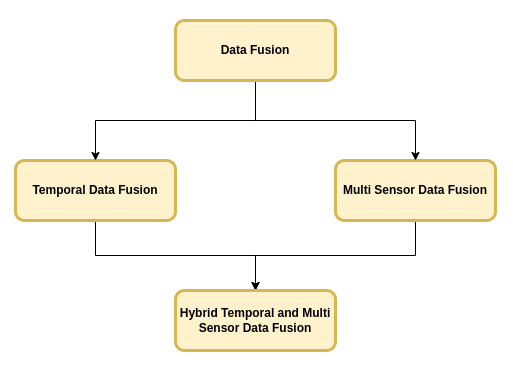
\includegraphics[width=10cm]{images/df.png}
		\caption{Data fusion categories based on the type of fusion. Temporal data fusion fuse the temporal data from past sequences, and multi-sensor data fuse the data from multiple sensors collected at the moment. Generated with \href{https://app.diagrams.net/}{Diagrams.net} }
		\label{fig:3D_reconstruction}
	\end{figure}

	Data fusion is divided into temporal and multi-sensor data fusion based on the timestamp factor. Temporal data are the data collected over time and fusing them together, resulting in temporal data fusion. In the multi-sensor data fusion approach, the data from different sensors are collected for a given time and fused for improved prediction. In the hybrid approach, temporal data and multi-sensor data are fused. Information fusion is applied in different fields such as time series prediction \cite{02_lim2021temporal}, video-based depth estimation \cite{03_duzceker2021deepvideomvs}, and segmentation \cite{04_li2021spatial}.
	
	Understanding the surrounding regions and the decision-making of a human is based on the signals obtained from different sensors. However, knowing the past helps to recognize the nearby activity better or make an educated choice. Fusing the information from different sources and the former data adds to an improved outcome. Temporal fusion fuses the information to the current step to improve the prediction at each timestamp. Common temporal data types include weather data, video sequence frames, and sensor data. Semantic segmentation takes advantage of temporal fusion to make a better decision. 
    
    \subsection{Temporal Fusion}
	
	In a general setting, the previous data is not utilized to make a current prediction, resulting in information loss. The rich features from the past can be utilized in the current step, thereby making a robust and efficient model prediction. Temporal fusion is one of the dimensions of data fusion, and different data sources collected over time are fused for improvement in the prediction \cite{005_hsiao2005temporal}. Classical multi-data fusion finds application in automatic target tracking, autonomous vehicle detection, surveillance systems, robotics, wearable devices, and manufacturing monitoring. The data is collected over time and contains essential features in all areas mentioned earlier. These temporal features are combined to make an efficient prediction. 
    
    The temporal fusion can model the behavioral aspect of the collected data rather than just the current timestep data. The temporal fusion extracts the relationship between contextual and temporal proximity \cite{07_hsiao2005temporal}. The temporal arrangements of events are captured, thereby incorporating the cause and effect phenomenon \cite{07_hsiao2005temporal}. Temporal fusion can be commonly observed in human activity detection \cite{08_krause2003unsupervised}, context-aware mobile phones [19], and online batch process monitoring \cite{09_lee2003line}. 
    
	A 3D object detection approach on two popular datasets, KITTI[4] and nuScenes[5] takes single-time step LIDAR data for prediction, resulting in the loss of valuable forecast and features computed during the previous step [3]. Using the rich features present in the successive frames to accommodate the past data at a time is extensively studied in neural network-based action recognition \cite{10_han2016seq} \cite{11_kang2017t} \cite{12_ning2017spatially} \cite{13_lu2020retinatrack} and video object detection \cite{14_kopuklu2019you} \cite{15_feichtenhofer2016convolutional} \cite{16_wang2016temporal} methods. The fusion of features from the previous step to the current step to improve the 3D object detection is studied in the Temp-Frustum Net architecture [3]. A Temporal Fusion Module (TFM) is proposed to combine the object-specific features. The temporal fusion method improved the average result by 6\% \cite{17_erccelik2021temp}. Depth maps using dynamic MRFs fuse Time-of-Flight (TOF) and passive stereo to get an enhanced depth map. The depth map estimation is extended to the temporal domain resulting in accurate depth maps \cite{18_zhu2009spatial}. Multi-camera video surveillance fuses the spatiotemporal frames from different sources to reliably find the motion trajectories \cite{19_wu2003multi}. A moving object is detected and segmented with the unmanned aerial vehicle (UAV) data by stacking the consecutive frames containing objects of interest resulting in constant object position and moving background, thereby improving the segmentation efficiency \cite{20_teutsch2012spatio}.

    \subsection{Semantic Segmentation}
	
	Segmentation of images is an essential task of visual understanding systems. It involves dividing the image into multiple segments. Image segmentation can be framed as classifying the individual pixels into a particular class or semantic labels. Segmentation can be classified as a semantic, instance, and panoptic. Segmentation of images finds a broad range of application areas \cite{21_forsyth2011computer}, such as medical for boundary extraction and tissue volume estimation, autonomous systems for detecting a boundary for path planning, and surveillance to track objects. Semantic segmentation is not only about the data but the problem segmentation addresses. For example, in a pedestrian detection system, pixels belonging to a person are categorized into a single class; however, for action recognition, the different parts of the body are classified into other classes. Instance segmentation \cite{22_dai2016instance} solves the problem of counting unique objects present in an image and is a common task in image retrieval tasks. Many traditional techniques have been developed to solve the segmentation problem \cite{23_fu1981survey}. For specialized tasks, different algorithms are developed \cite{24_ladys1994colour}. Work by Shervin surveyed the various state-of-the-art segmentation algorithms \cite{25_minaee2021image}. However, many algorithms are developed, but only some works are proposed for multi-view semantic segmentation. From the previous work, it is evident that temporal fusion improves the model's performance. This work aims to study the impact of the temporal fusion of information in the latent space and cross-transfer the technology to the semantic segmentation task. 

    \section{Challenges and Difficulties}
    
	Deep learning methods have contributed to the improvement of semantic segmentation. Building a temporal fusion for a semantic segmentation model is challenging due several factors involved such as temporal variations, handling large data volumes, noise and error corrections, robustness to different scenarios. Common challenges involved are the 
   
    \begin{itemize}
    	\setlength\itemsep{0.01em}
    	\item Datasets
    	\item Fusion architecture
    	\item Computation cost
    	\item Application areas
    \end{itemize}
	
		
    \subsection{Dataset}
	
	The deep learning model can be trained from scratch in many application areas, given that we have large datasets. However, there are not enough datasets available for a new domain to train the model; in such cases, transfer learning can be applied. In the transfer learning approach, a model is trained on some data, and the part of trained model weights are used for building a new application areas architecture. Many deep learning-based models are trained on the ImageNet datasets and take the pretrained encoder weights, which capture the features needed to do the segmentation, thereby reducing the dependency on the requirement of large datasets. Image augmentation is another approach to increase the number of data points. Data augmentation helps to create more data by applying a transformation to the existing small datasets so that a variety of input data is generated from the existing small datasets. Some typical transformations on the input images are translation, reflection, rotation, warping, scaling, color space shifting, and projecting onto the principal component. It helps to faster convergence, reduce the over-fitting probability, and improve the model's generalization capability. For some tasks, data augmentation showed improvement in the model's performance. For temporal fusion, there is a need for 2D datasets along with the camera's pose. Pose information can be fused at the latent space to improve the prediction efficiency of the model. There is a need for different kinds of datasets, such as still images, navigation datasets, and Unmanned aerial vehicle (UAV) datasets, to validate the model in a different environment, and helps to evaluate the model performance.  

    \subsection{Fusion Architecture}
    
    With the advancement of deep learning, more segmentation models are developed with improved efficiency and a variety of fusion architecture. The fusing of features is commonly used in the segmentation task. Adapting fusion features in the increased depth deep learning model showed significant improvement in the prediction. U-Net \cite{26_ronneberger2015u} model effectively use the already learned features by fusing the information from the encoder to the decoder. To tackle the decrease of initial image resolution at the output, a RefineNet \cite{27_lin2017refinenet} network was proposed. Deeper layers capture the high-level semantic features refined by fusing the fine-grained features from the earlier convolutions. Dense connection is employed in many of the recent neural network architectures \cite{28_jegou2017one}, \cite{29_iandola2014densenet}, \cite{30_yang2018denseaspp}. Choosing the appropriate fusion architecture depends on the problem and the available resources to solve the problem. 

    \subsection{Computation Cost}
    
    Many state-of-the-art segmentation networks require high computation costs during training and inference time. So the recent research is focused on decreasing the computation cost and keeping the model's accuracy high. To deploy the model in low computational mobile devices, simpler models need to be developed that fit the device's computation cost. This can be done by compressing the model or using the knowledge distillation techniques to build the low computational model \cite{25_minaee2021image}. 
    
    \subsection{Real Time Inference for Various Application Areas}
	
	Most of the recent top-performing semantic segmentation models are based on the fully convolutional network \cite{31_chen2014semantic}. A real-time application or the camera's frame rate needs to be high, and the model has reasonable accuracy and prediction speed. Real-time prediction is highly critical in the autonomous driving and medical fields. However, most of the fully convolutional network needs to be better with respect to the maximum requirements defined by application areas. Models with dilated convolution improved the performance of the model. However, the benchmark can still be improved. ICNet takes multiple input sizes to capture objects of varying sizes to tackle the real-time deployment \cite{32_zhao2018icnet}.       

	\section{Use Cases}
	
	Semantic segmentation finds application in many areas of computer vision. Some of them are listed below,
	\subsection{Autonomous Driving and Robotics}
	
	Essential components of autonomous driving systems are object recognition, object localization, and segmentation. Semantic segmentation classifies each image pixel into a particular class, thereby identifying different classes such as street, traffic signs, trees, cars, sky, pedestrians, or sidewalks. Due to safety concerns, it is critical to classify each pixel with high accuracy. The rich information captured in the last step can be used in the current step calculation to make a better prediction at the current computational step. With the development of the robotics system to perform complex tasks, the interaction with the environment also increased. So, there is a need to develop a robust system to understand the knowledge about the workspace. 
	 
	\subsection{Weed Mapping Using Unmanned Aerial Vehicle (UAV)}
	
	Mapping of the fields is essential for weed control and spraying applications. The presence of the weed can be mapped by unmanned aerial vehicle remote sensing technology. The targeted spraying of the weed area helps to curb weed growth by inspecting the weed map obtained from the UAV. The entire process involves real-time image processing hardware that integrates map visualization, flight control; image collection \cite{33_deng2020lightweight}. Semantic segmentation can be employed with good performance and real-time capability to build a weed map. 
	
	\subsection{Real-Time Hand Gesture Recognition}
	
	Hand Gesture Recognition (HGR) is an essential component in human-computer interactions. With the advancement of vision-based HGR systems, HGR is widely used in the automotive sector, consumer electronics, home automation, etc. An essential feature of the HGR is real-time performance, and HGR should perform without lag to control the cursor's location. HGR is based on the semantic segmentation method to locate the hand's position; therefore, an efficient real-time segmentation network needs to be developed \cite{34_hsieh2010real}.  
	
	\vspace{65mm} %5mm vertical space
	
    \section{Problem Statement and Contribution}
    
    Research question answered and contribution in the thesis work is listed below
    \subsection{Research Questions}
    
     \begin{itemize}
    	\setlength\itemsep{0.01em}
    	\item[RQ1] What are the works on state-of-the-art temporal fusion?
    	\item[RQ2] How are the results from RQ1 compared with each other to perform temporal
    	fusion?
    	\item[RQ3] How to cross-transfer the depth estimation temporal fusion technique to semantic segmentation?
    \end{itemize}
    
    \subsection{Contributions}
    
    \begin{itemize}
    	\item Literature review on the temporal fusion in the context of depth estimation and semantic segmentation
    	\item Analysis of the state-of-the-art temporal fusion architectures
    	\item Create a baseline of temporal fusion with sequence images
    	\item  Compare performances of state-of-the-art temporal fusion techniques with different error metrics
    	\item Cross-transfer the temporal fusion architecture to the segmentation task
  
	\end{itemize}
    \section{Report Outline}
    
    The theoretical background of deep learning, semantic segmentation, temporal fusion, and their limitations is discussed in Chapter \ref{chap:stateofart}. Datasets, preprocessing steps, experimental designs, training procedures, and hardware configuration used for training and inferences are listed down in Chapter \ref{chap:methodology}. Evaluation of the temporal fusion architecture with different experimental settings, metrics, and research questions are discussed in Chapter \ref{chap:evaluationandresult}. Deployment of the model in the android is described in the android deployment Chapter \ref{chap:androiddeploy}. Finally contribution of the thesis work, lessons learned, and future work is explained in conclusion chapter \ref{chap:conclusion}. 
    
